\section{About Graphs}
\begin{frame}
	\frametitle{Graph Theory}
	\begin{itemize}
		\item Powerful tool for modeling
			\begin{itemize}
				\item Relations
				\item Processes
			\end{itemize}
		\item Examples
			\begin{description}
				\item [Social network:] Vertex: person, Edge: friendship relation
				\item [Neuroscience:] Modeling neural network~\footcite{BuSp09}
				\item [Telecommunications:] Peer-to-peer mobile networks~\footcite{FaCh99}
			\end{description}
	\end{itemize}
\end{frame}

\begin{frame}
	\frametitle{Undirected simple Graphs}
	\begin{itemize}
		\item Formal Description
			\begin{itemize}
				\item $G = (V,E)$
				\item $V$ an unordered set of vertices
				\item $E$ an unordered set of unordered pairs $\{u,v\}, u \in V, v \in V$
			\end{itemize}
	\end{itemize}
	\begin{figure}
		\begin{center}
			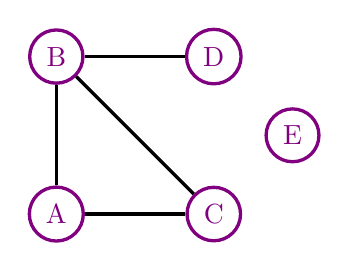
\begin{tikzpicture}[scale=0.5]
  \node[draw,circle, very thick, color=violet] (A) at (2,0) {A};
  \node[draw,circle, very thick, color=violet] (B) at (2,4) {B};
  \node[draw,circle, very thick, color=violet] (C) at (6,0) {C};
  \node[draw,circle, very thick, color=violet] (D) at (6,4) {D};
  \node[draw,circle, very thick, color=violet] (E) at (8,2) {E};
  \draw[very thick] (A) -- (B);
  \draw[very thick] (B) -- (D);
  \draw[very thick] (C) -- (B);
  \draw[very thick] (C) -- (A);
\end{tikzpicture}

		\end{center}
		\caption{An undirected simple graph with 5 vertices and 4 edges}
	\end{figure}
\end{frame}


